\section{Kodelås (Philip)} \label{sec:Kodelaas}

I dette afsnit testes hvorvidt kommunikationen mellem Altera DE2 boardet og Atmel STK500 kittet virker.

Vhdl filen for kodelåsen \cite{lib:Codelock} downloades til DE2 boardet og der monteres et et Analog discovery oscilloskop på DE2 boardets GPIO(1) pin 0 med en reference på GPIO(1) pin 11(GND).

\begin{figure}[h]
	\centering
	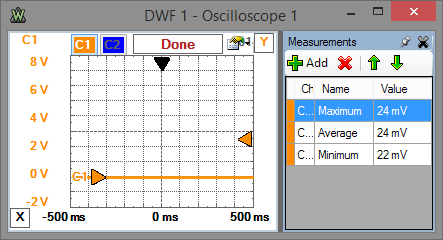
\includegraphics[scale=1, trim=0 0 0 0, clip=true]{../Implementering/billeder/DE2LOW.png}
	\caption{Analog discovery - Oscilloskop: DE2 LOW output}
	\label{fig:DE2LOW}
\end{figure}

\begin{figure}[h]
	\centering
	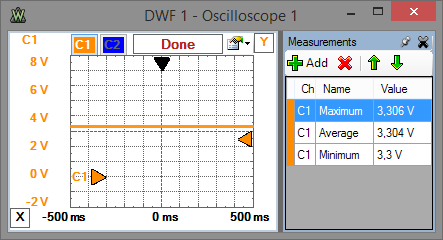
\includegraphics[scale=1, trim=0 0 0 0, clip=true]{../Implementering/billeder/DE2HIGH.png}
	\caption{Analog discovery - Oscilloskop: DE2 HIGH output}
	\label{fig:DE2HIGH}
\end{figure}

På figur \ref{fig:DE2LOW} og \ref{fig:DE2HIGH} kan det ses at et logisk HIGH output på DE2 boardet er målt til en spænding på $3.3V$ og en logisk LOW har en spænding på $0.0V$.

For at teste om dette er en spænding der er høj nok til at STK500-kittet registrer det som HIGH, laves et lille testprogram. Testprogrammet sætter $PORT C$ LOW, når $PORT A$ pin 0 sættes HIGH og omvendt.

\begin{lstlisting}
#include <avr/io.h>

void main(void)
{
	DDRA = 0x00;	// PORTA is input
	DDRC = 0xFF;	// PORTC is output
	
	while(1)
	{
		if (PINA==0b00000001)	// Read PORT A0 and checks if it is HIGH
		{
			PORTC = 0x00;		// LEDs turns on (PORTC is LOW)
		}
		else
		{
			PORTC = 0xFF;		// LEDs turns off (PORTC is HIGH)
		}
	}
}
\end{lstlisting}

Med en Analog discovery's funktionsgenerator laves et sinussignal med en amplitude på 5V som sættes til $PORT A$ pin 0. Med analog discovery's oscilloskop måles nu på et tilfældig ben på $PORT C$.

\begin{figure}[h]
	\centering
	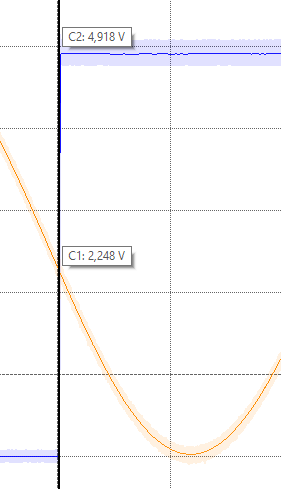
\includegraphics[scale=0.7, trim=0 0 0 0, clip=true]{../Implementering/billeder/STK_FALING.png}
	\caption{Analog discovery - Oscilloskop: STK-500 Faling edge}
	\label{fig:STK_FALING}
\end{figure}

Det ses på figur \ref{fig:STK_FALING} at der skal påtrykkes en spænding på $2.3V$ for at STK500-kittet til at skifter fra at registrere HIGH til at registrere LOW.

\begin{figure}[h]
	\centering
	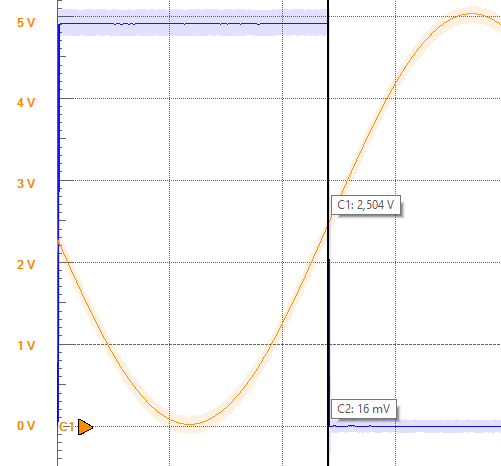
\includegraphics[scale=0.7, trim=0 0 0 0, clip=true]{../Implementering/billeder/STK_RISING.png}
	\caption{Analog discovery - Oscilloskop: STK-500 Rising edge}
	\label{fig:STK_RISING}
\end{figure}

Det ses på figur \ref{fig:STK_RISING} at der skal påtrykkes en spænding på $2.5V$ for at STK500-kittet til at skifter fra at registrere LOW til at registrere HIGH.


%% \textcolor{red}{http://www.atmel.com/images/doc2503.pdf side 287}\\

%% I databladet for At mega32, som er den microchip der sidder på STK500-kittet, er det angivet at for at et indput registreres som HIGH, skal det have en spænding på min $V_{CC}\cdot0.6V$ og max $V_{CC}+0.5V$\\

%% \textcolor{red}{(udregning)}\\

For at kunne udføre en samlet modultest, tilsluttes STK500-kittet PORT A pin 0 til DE2 boardets GPIO(1) pin 0 og et GND-ben på STK500-kittet tilsluttes GPIO(1) pin 11. Ydermere tilsluttes STK500-kittet PORT C til dets indbyggede LED'er.

På både STK500-kittet og DE2 boardet ligger samme software som i de ovenstående test. Det kan nu ses at STK500-kittets LED'er tænder og slukker som forventet, alt efter kom koderne på DE2-boardet er indtastet korrekt.

Altså er kan det konkluderes at vi godt kan bruge koble DE2 boardet direkte til STK500-kittet.